\documentclass[conference]{IEEEtran}
\usepackage[T1]{fontenc}
\usepackage{amsmath}
\usepackage{booktabs}
\usepackage{tabularx}
\usepackage{tikz}
\usepackage[hidelinks]{hyperref}
\usetikzlibrary{arrows.meta}
\newcolumntype{L}{>{\raggedright\arraybackslash}X}

% Replace these fields before submission.
\newcommand{\studentname}{Student Name(s)}
\newcommand{\department}{Department and Institution}
\newcommand{\studentemail}{Roll Number(s) and Email Address(es)}

\title{SoilWise: Explainable Crop Recommendation and Soil Screening from Manual Inputs and Lab Reports}
\author{\IEEEauthorblockN{\studentname}
\IEEEauthorblockA{\department\\\studentemail}}

\begin{document}
\maketitle

\begin{abstract}
Soil test results and weather observations can inform crop selection, but the inputs may arrive as separate measurements or as laboratory documents that require manual transcription. SoilWise is a web prototype that screens soil measurements and recommends crops from seven soil and climate inputs. The application accepts manual entry or extracts candidate values from PDF and image reports for user review. A rules service screens pH and nutrients, while a supervised classifier ranks three crop labels, explains the leading result with SHAP, and displays a K-means cluster for context. We compared a majority baseline, Decision Tree, Random Forest and XGBoost on a public benchmark of 2,200 records covering 22 balanced crop classes. With a fixed stratified 80/20 split, Random Forest achieved the highest repeated validation macro-F1 of 0.9932. After nested tuning, the selected pipeline classified 438 of 440 held-out records correctly. Its test accuracy and macro-F1 were both 0.9955, and its macro one-vs-rest AUC was 1.0000. Training-fold ablation found that removing rainfall caused the largest drop among the inputs tested. A React interface and FastAPI service support the workflow. Field suitability and extraction reliability across laboratory report formats require independent validation.
\end{abstract}

\begin{IEEEkeywords}
crop recommendation, soil screening, Random Forest, SHAP, optical character recognition, precision agriculture
\end{IEEEkeywords}

\section{Introduction}
Crop selection involves soil nutrient status, acidity and climate. A laboratory report may provide nutrient and pH values while leaving rainfall, temperature and humidity to the user. Our objective was to build a repeatable workflow that can interpret the readings available, request the remaining values needed for classification, and show the basis of each result. The interface includes Maharashtra demonstration profiles. Location and farming context are stored as descriptive metadata.

SoilWise combines three outputs. Rule-based screening rates available soil measurements. Supervised learning ranks crop labels once all seven features are present. Unsupervised clustering places the input among similar benchmark profiles. The application also shows missing fields, tracks whether values were marked measured or estimated, and allows users to verify extracted report values before submitting them.

\section{Related Work and Research Gap}
Table~\ref{tab:literature} compares ten recent studies. Indian tabular-data studies establish useful classifier benchmarks, while other work explores ensemble design, explanations, and interaction. The cloud and multimodal systems demonstrate that crop recommendation can extend beyond an offline comparison. Across the studies reviewed, verified transcription from laboratory documents and explicit handling of a mismatch between laboratory nutrient units and the classifier's input scale received less attention. SoilWise addresses that application gap with editable extraction, two nutrient screening modes and a warning when lab-scale values are used for classification. Its contribution is the integrated workflow and its documented behavior with incomplete inputs.

\begin{table}[t]
\caption{Recent work on crop recommendation}
\label{tab:literature}
\centering\footnotesize
\begin{tabularx}{\columnwidth}{@{}p{.24\columnwidth}L@{}}
\toprule
Study & Method and relevance to SoilWise \\
\midrule
Thilakarathne et al. \cite{cloud} & Demonstrates machine-learning crop selection in a hosted interface. \\
Elbasi et al. \cite{elbasi} & Benchmarks 15 algorithms and examines feature combinations. \\
Dey et al. \cite{dey} & Compares classifiers for Indian crops using NPK, pH and climate. \\
Prity et al. \cite{springer} & Compares nine classifiers on the 22-crop dataset. \\
Bouni et al. \cite{interpretable} & Combines Random Forest with SHAP and LIME for local interpretation. \\
Afzal et al. \cite{afzal} & Studies benchmark features and soil information for crop prediction. \\
Stracqualursi \cite{stracqualursi} & Evaluates exponential reweighting of several classifiers. \\
Bakr et al. \cite{mdpi} & Compares tabular models with GPT-2 for conversational access. \\
Sahu and Sujithra \cite{sahu} & Fuses soil imagery, sensor readings and weather inputs. \\
Dhiyanesh et al. \cite{deep} & Applies SHAP to a crop model combining Transformer, GRU and feed-forward layers. \\
\bottomrule
\end{tabularx}
\end{table}

\section{Methodology and Experimental Setup}
Figure~\ref{fig:training-flow} summarizes how the split keeps model selection and final evaluation separate.

\begin{figure}[t]
\centering
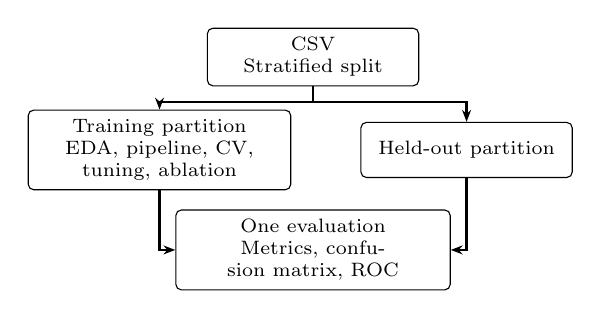
\begin{tikzpicture}[font=\scriptsize,
  block/.style={draw,rounded corners=2pt,align=center,text width=2.45cm,minimum height=7mm},
  connection/.style={-{Stealth[length=1.5mm]},thick}]
\node[block] (split) at (0,0) {CSV\\Stratified split};
\node[block,text width=3.10cm] (train) at (-1.95,-1.18) {Training partition\\EDA, pipeline, CV, tuning, ablation};
\node[block] (test) at (1.95,-1.18) {Held-out partition};
\node[block,text width=3.25cm] (eval) at (0,-2.45) {One evaluation\\Metrics, confusion matrix, ROC};
\draw[connection] (split.south) -- ++(0,-2mm) -| (train.north);
\draw[connection] (split.south) -- ++(0,-2mm) -| (test.north);
\draw[connection] (train.south) |- (eval.west);
\draw[connection] (test.south) |- (eval.east);
\end{tikzpicture}
\caption{Offline workflow. Candidate selection and ablation use training data. The fitted winner and test partition meet at the final evaluation.}
\label{fig:training-flow}
\end{figure}

\subsection{Stage 1. Data and Exploratory Analysis}
We used a copy of the Crop Recommendation Dataset \cite{dataset} from the Harvestify mirror documented in the repository. It contains 2,200 records, seven numeric predictors and one crop label. Each of the 22 classes has 100 records. The integrity script found zero missing cells and zero duplicate rows. The workflow records training feature summaries, correlations, class counts and counts beyond 1.5 interquartile ranges. We retained the flagged points because an unusual value within a mixed-crop dataset can be legitimate.

The training partition contains 80 records per crop. Table~\ref{tab:data} summarizes its feature values. Figure~\ref{fig:eda} shows the strongest training correlations by absolute value. The P--K correlation of 0.736 motivates checking how the forest performs when K is removed. The dataset documentation leaves NPK units unspecified and supplies no site coordinates or dates.

\begin{table}[t]
\caption{Training feature summary and integrity checks}
\label{tab:data}
\centering\footnotesize
\begin{tabular}{@{}lrrr@{}}
\toprule
Feature & Mean $\pm$ SD & Range & IQR flags \\
\midrule
N & $50.55\pm36.86$ & 0--140 & 0 \\
P & $53.34\pm32.95$ & 5--145 & 108 \\
K & $48.14\pm50.71$ & 5--205 & 160 \\
Temperature ($^\circ$C) & $25.61\pm5.08$ & 8.83--43.68 & 72 \\
Humidity (\%) & $71.42\pm22.28$ & 14.26--99.98 & 24 \\
pH & $6.47\pm0.78$ & 3.50--9.94 & 43 \\
Rainfall (mm) & $103.45\pm54.99$ & 20.21--298.56 & 82 \\
\bottomrule
\end{tabular}
\end{table}

\begin{figure}[t]
\centering
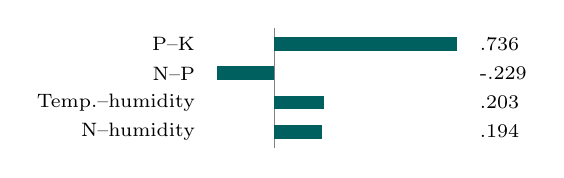
\begin{tikzpicture}[x=3.15cm,y=.37cm,font=\scriptsize]
\draw[gray] (0,.45)--(0,4.55);
\foreach \y/\lab/\v in {4/P--K/.736,3/N--P/-.229,2/Temp.--humidity/.203,1/N--humidity/.194}{
  \node[anchor=east] at (-.28,\y) {\lab};
  \draw[teal!75!black,line width=5pt] (0,\y)--(\v,\y);
  \node[anchor=west] at (.79,\y) {\v};
}
\end{tikzpicture}
\caption{Four largest absolute Pearson correlations on the training data. The N--P bar extends left of zero.}
\label{fig:eda}
\end{figure}

\subsection{Stage 2. Stratified Split}
The split in \texttt{ml/preprocessing.py} uses \texttt{train\_test\_split} with seed 42, \texttt{stratify=y} and test fraction 0.20. The resulting training and test sets contain 1,760 and 440 records, respectively. Every test class has 20 records. Candidate comparison, tuning, ablation and clustering use training rows. The metrics store the split settings and a SHA-256 digest of the CSV. This benchmark retains the same deterministic partition as the earlier project version.

\subsection{Stage 3. Preprocessing}
The classifier consumes seven numeric features in the saved order N, P, K, temperature, humidity, pH and rainfall. The workflow fits \texttt{LabelEncoder} on training labels to map crop names to stable IDs. A scikit-learn \texttt{Pipeline} contains a median \texttt{SimpleImputer}, \texttt{StandardScaler} and classifier \cite{sklearn}. Each fit learns its medians and scaler statistics from the training rows in that fold. The current CSV is complete, so imputation leaves the existing values intact. Equal class counts allow the workflow to use the original class distribution. The Joblib bundle stores the fitted pipeline, feature order and label mapping.

The clustering branch fits its imputer and scaler on training features because K-means uses Euclidean distance. It compares $k=2$ through $8$ using silhouette score, with 10 initializations and seed 42 per fit. The best score is 0.4158 at $k=2$. Crop labels summarize clusters after fitting. PCA projects a 300-record training sample and the current input into two dimensions for display.

\subsection{Stage 4. Baselines and Comparison}
The Decision Tree provides a single-tree comparison. Random Forest uses 300 trees to average predictions across randomized trees \cite{breiman}. The XGBoost candidate uses 200 boosting rounds, depth 5, learning rate 0.1 and multiclass log loss \cite{xgboost}. The training script repeats stratified five-fold validation twice with seed 42 and selects the trained model family with the highest mean macro-F1. A \texttt{DummyClassifier} with \texttt{most\_frequent} provides a reference. With equal counts, its accuracy equals $1/22$.

\subsection{Stage 5. Hyperparameter Tuning}
After the repeated comparison selected Random Forest, its grid search fixed the tree count at 300 and varied maximum depth $\{\text{unlimited},12\}$ and minimum samples per leaf $\{1,2\}$. Three shuffled inner stratified folds (seed 42) optimize macro-F1. Three outer stratified folds (seed 43) assess the search within the selected model family. A search on all training rows selects the settings and refits the production pipeline. The outer score is conditional on the family chosen during the repeated comparison.

\subsection{Stage 6. Feature Ablation}
We retrained the chosen pipeline with the tuned parameters held fixed and removed rainfall, humidity and K one at a time. We used the same five stratified training folds and seed across conditions. The differences in mean macro-F1 measure dependence on each input within this dataset and model. Correlated inputs can supply overlapping information.

\subsection{Stage 7. Held-out Evaluation}
A single \texttt{predict\_proba} call on the selected pipeline supplies held-out class scores. The highest score gives the predicted label for accuracy, macro precision, macro recall, macro-F1 and the confusion matrix. The same scores produce 22 one-vs-rest ROC curves. Macro AUC averages their areas with equal weight. The micro-average curve pools all sample--class decisions. The project saves these outputs for the selected pipeline in \texttt{backend/saved\_models/metrics.json}.

\subsection{Stage 8. Delivery and Explainability}
The application joins a Vite/React TypeScript frontend to FastAPI. Figure~\ref{fig:flow} shows how the two input paths meet at validation. The shipped artifacts contain the fitted classifier pipeline, clustering preprocessing, clusterer, PCA background sample, and evaluation metrics. During inference, \texttt{predict\_proba} ranks the top three crop labels. SHAP TreeExplainer uses the classifier's preprocessed inputs and assigns a signed contribution to each feature for the leading crop \cite{shap}. The interface shows these contributions and the cluster plot with the model version, training-range warnings and input provenance.

\begin{figure}[t]
\centering
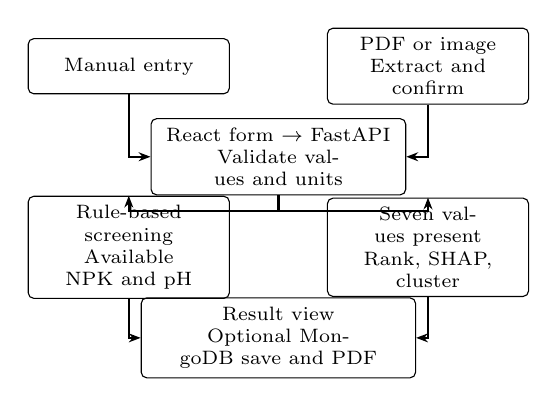
\begin{tikzpicture}[font=\scriptsize,
  box/.style={draw, rounded corners=2pt, align=center, minimum height=7mm, text width=2.32cm},
  edge/.style={-{Stealth[length=1.5mm]},thick}]
\node[box] (manual) at (-1.9,0) {Manual entry};
\node[box] (report) at (1.9,0) {PDF or image\\Extract and confirm};
\node[box,text width=3cm] (api) at (0,-1.15) {React form $\rightarrow$ FastAPI\\Validate values and units};
\node[box] (screen) at (-1.9,-2.30) {Rule-based screening\\Available NPK and pH};
\node[box] (model) at (1.9,-2.30) {Seven values present\\Rank, SHAP, cluster};
\node[box,text width=3.25cm] (out) at (0,-3.45) {Result view\\Optional MongoDB save and PDF};
\draw[edge] (manual.south) |- (api.west);
\draw[edge] (report.south) |- (api.east);
\draw[edge] (api.south) -- ++(0,-2mm) -| (screen.north);
\draw[edge] (api.south) -- ++(0,-2mm) -| (model.north);
\draw[edge] (screen.south) |- (out.west);
\draw[edge] (model.south) |- (out.east);
\end{tikzpicture}
\caption{SoilWise request flow. Incomplete submissions take the screening path and receive a message listing the inputs needed for crop ranking.}
\label{fig:flow}
\end{figure}

\section{How SoilWise Works}
\subsection{Manual Entry and Soil Screening}
The user enters measured or estimated soil and climate values, selects the NPK unit convention, and can add a location and farming context. React checks the numeric bounds and sends the form to \texttt{POST /api/soil/analyze}. Pydantic validates the request before calling the analysis service. The soil screening service marks missing nutrients and assigns pH to one of five acidity categories. It uses dataset terciles for dataset-scale NPK, or hard-coded general lab thresholds for kg/ha. Those thresholds provide coarse screening; the form bounds also limit the accepted range of lab N. The application supplies general follow-up advice without a fertilizer dose.

When all seven features are supplied, the service builds a one-row data frame in the saved feature order, runs the classifier and attaches its explanation and cluster. A permitted input outside the stored dataset ranges triggers an extrapolation warning. A kg/ha submission can still receive a crop ranking, with a warning that the model's undocumented NPK scale makes that ranking unreliable. The application performs no unit conversion.

\subsection{Laboratory Document Entry}
\texttt{POST /api/soil/upload-report} checks the upload size, extension and file signature. PDF, JPG, JPEG and PNG are accepted. The default API limit is 5 MB. PyMuPDF extracts a PDF's embedded text when available. Otherwise the service renders scanned pages and prepares them or uploaded images with OpenCV grayscale conversion, upscaling, denoising and adaptive thresholding before Tesseract OCR \cite{tesseract}. Regular expressions look for N, P, K, pH, organic carbon and electrical conductivity. The form imports detected NPK and pH; organic carbon and electrical conductivity are extraction metadata and outside the prediction feature set. The user can edit the suggestions, add weather observations and confirm the extracted values before submitting. The service persists no original file.

\subsection{Interface, Storage, and PDF Generation}
The frontend includes a dashboard, an analysis form, history with side-by-side comparisons, and a model page. The model page shows class balance, correlations, candidate results, tuning, ablation, ROC, the confusion matrix and cluster summaries. The dashboard draws saved-record statistics such as crop frequencies and pH categories. With MongoDB configured, the service stores an analysis ID, timestamp, input values, source labels and model output. A saved record can be reopened or deleted. The report endpoint builds a downloadable PDF from the stored record using ReportLab. Without a database, the analysis still returns and the response indicates whether saving was possible. History, dashboard statistics and saved reports return HTTP 503 when persistence is unavailable.

\section{Results and Discussion}
\subsection{Classifier Performance}
Table~\ref{tab:official} reports the selected pipeline's held-out scores. It correctly classified 438 records. It confused one blackgram record with maize and one rice record with jute (Fig.~\ref{fig:cm}). The other 20 classes each had 20 correct predictions. Across records, each one-vs-rest curve perfectly separates its class on this split. Within an individual record, taking the largest score across classes can still select the wrong crop. Figure~\ref{fig:roc} shows the small false-positive-rate region where the pooled ROC reaches full recall.

\begin{table}[t]
\caption{Selected Random Forest on 440 held-out records}
\label{tab:official}
\centering\scriptsize
\begin{tabular}{@{}lr@{}}
\toprule
Metric & Value \\
\midrule
Accuracy & 0.9955 \\
Macro precision & 0.9957 \\
Macro recall & 0.9955 \\
Macro-F1 & 0.9955 \\
Macro one-vs-rest AUC & 1.0000 \\
Micro one-vs-rest AUC & 0.999996 \\
\bottomrule
\end{tabular}
\end{table}

\begin{figure}[t]
\centering
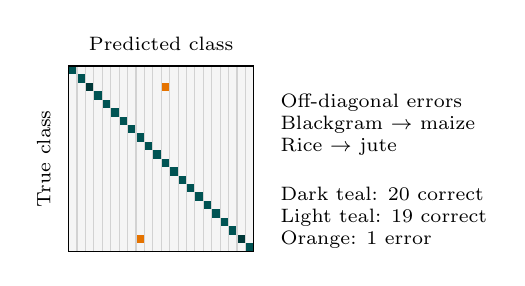
\begin{tikzpicture}[x=.107cm,y=-.107cm,font=\scriptsize]
\fill[gray!8] (0,0) rectangle (22,22);
\foreach \i in {0,...,21}{\fill[teal!65!black] (\i,\i) rectangle ++(1,1);}
\foreach \i in {2,20}{\fill[teal!44!black] (\i,\i) rectangle ++(1,1);}
\foreach \row/\col in {2/11,20/8}{\fill[orange!90!black] (\col,\row) rectangle ++(1,1);}
\draw[gray!35,step=1] (0,0) grid (22,22);
\draw (0,0) rectangle (22,22);
\node[anchor=south] at (11,-.7) {Predicted class};
\node[rotate=90,anchor=south] at (-1,11) {True class};
\node[anchor=west,align=left] at (24,7) {Off-diagonal errors\\Blackgram $\to$ maize\\Rice $\to$ jute};
\node[anchor=west,align=left] at (24,18) {Dark teal: 20 correct\\Light teal: 19 correct\\Orange: 1 error};
\end{tikzpicture}
\caption{Random Forest confusion matrix on 440 test rows, with crops ordered alphabetically by the saved label mapping.}
\label{fig:cm}
\end{figure}

\begin{figure}[t]
\centering
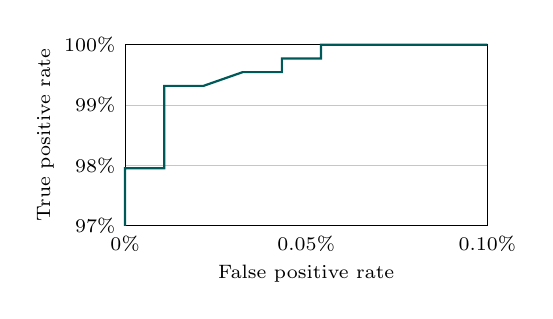
\begin{tikzpicture}[x=4.6cm,y=2.3cm,font=\scriptsize]
\foreach \y/\ticktext in {0/97,0.3333/98,0.6667/99,1/100}{
  \draw[gray!45] (0,\y)--(1,\y);
  \node[left] at (0,\y) {\ticktext\%};
}
\draw (0,0) rectangle (1,1);
\draw[teal!70!black,thick] plot coordinates {
  (0,0) (0,.3182) (.1082,.3182) (.1082,.7727) (.2165,.7727)
  (.3247,.8485) (.4329,.8485) (.4329,.9242) (.5411,.9242)
  (.5411,1) (1,1)
};
\foreach \x/\ticktext in {0/0,.5/0.05,1/0.10}{
  \node[below] at (\x,0) {\ticktext\%};
}
\node[below] at (.5,-.16) {False positive rate};
\node[rotate=90] at (-.22,.5) {True positive rate};
\end{tikzpicture}
\caption{Micro-average ROC zoom near the optimal corner. The complete curve and the per-class curves are saved in the metrics.}
\label{fig:roc}
\end{figure}

\subsection{Repeated Validation, Tuning, and Ablation}
Table~\ref{tab:repeated} reports ten validation folds. The majority-class baseline establishes how a constant prediction scores on the balanced dataset. The standard deviations describe variability across folds. Candidate comparison and ablation both use training data.

The nested search achieved outer accuracy of $0.9955\pm0.0021$ and outer macro-F1 of $0.9954\pm0.0022$. Its winning depth and minimum leaf size varied across outer folds. The full training search selected unlimited depth and a minimum of one sample per leaf, with inner macro-F1 of 0.9937.

Removing rainfall reduced macro-F1 by 0.0297, the largest drop in Table~\ref{tab:ablation}. Removing humidity reduced it by 0.0097, while removing K reduced it by 0.0046. Differences in impurity importance and ablation impact can arise when features contain overlapping predictive information, as P and K do in this split.

\begin{table}[t]
\caption{Repeated training CV ($2\times5$ folds)}
\label{tab:repeated}
\centering\footnotesize
\begin{tabular}{@{}lcc@{}}
\toprule
Model & Accuracy mean $\pm$ SD & Macro-F1 mean $\pm$ SD \\
\midrule
Majority class & $.0455\pm.0000$ & $.0040\pm.0000$ \\
Decision Tree & $.9841\pm.0065$ & $.9840\pm.0065$ \\
Random Forest & $.9932\pm.0046$ & $.9932\pm.0046$ \\
XGBoost & $.9901\pm.0071$ & $.9900\pm.0072$ \\
\bottomrule
\end{tabular}
\end{table}

\begin{table}[t]
\caption{Random Forest ablation on five training folds}
\label{tab:ablation}
\centering\footnotesize
\begin{tabular}{@{}lcc@{}}
\toprule
Input features & Macro-F1 mean $\pm$ SD & $\Delta$ F1 \\
\midrule
All seven & $.9931\pm.0053$ & 0.0000 \\
Without rainfall & $.9634\pm.0038$ & $-0.0297$ \\
Without humidity & $.9834\pm.0056$ & $-0.0097$ \\
Without K & $.9886\pm.0060$ & $-0.0046$ \\
\bottomrule
\end{tabular}
\end{table}

\subsection{Verification and Limitations}
The current backend test run passed 12 cases and skipped the PNG OCR case because Tesseract was unavailable on PATH. Passing cases covered the held-out metrics and ROC, the rice ranking and SHAP result, input rejection, partial-input screening, embedded PDF text extraction, rejected uploads, and mock-database save, retrieval, statistics, PDF export and deletion. The Vite production build passed, and a fresh FastAPI/Vite smoke test returned results through the frontend proxy. OCR on diverse real lab reports, live Atlas persistence and mobile browser behavior lack verification.

The curated benchmark is balanced and highly separable. The split tests interpolation within the same data source. Without coordinates or dates, it cannot test transfer to a new district or growing season, and the interface's location field does not alter inference. Class scores are useful for ranking, with no calibration study or measured yield outcomes. The pH and nutrient rules provide an initial interpretation; local fertilizer and soil treatment decisions require laboratory and agronomic context. Shared deployments also need user authentication and authorization for saved records.

\section{Reproducibility and Rubric Evidence}
The public \href{https://github.com/hari-02006/soilwise-backend}{SoilWise GitHub repository} has a history covering initial implementation, API proxy configuration and dependency setup. The hosted demo is at \url{https://soilwise-frontend.onrender.com}. A local demo is available at \url{http://localhost:5173} while the application is running. API documentation is at \url{http://localhost:8000/docs}.

Install the backend dependencies from \texttt{backend/requirements.txt}. In the backend, run \texttt{python -m ml.train} to regenerate model artifacts, \texttt{python -m pytest -q} to test, and \texttt{python -m uvicorn app.main:app --reload} to start the API. In the frontend, run \texttt{npm install} followed by \texttt{npm run dev}. Tesseract on PATH enables scan recognition. Set \texttt{MONGODB\_URI} in \texttt{backend/.env} to enable persistence. For a demonstration, submit N=90, P=42, K=43, pH=6.5, temperature=20.9, humidity=82 and rainfall=203 on the dataset scale. The API test verifies that rice ranks first for this example. Next submit pH=5.0 and N=20 alone to show partial screening.

\begin{table}[t]
\caption{Implementation marking criteria and evidence}
\label{tab:rubric}
\centering\footnotesize
\begin{tabularx}{\columnwidth}{@{}p{.29\columnwidth}L@{}}
\toprule
Criterion & Project and report evidence \\
\midrule
Data handling (4) & \texttt{ml/preprocessing.py}, fixed split, fold-fitted pipeline, integrity table and training EDA. \\
Model building (4) & Three trained candidates and a majority baseline compared by repeated stratified CV in \texttt{ml/train.py}. \\
Tuning and validation (4) & Seeded nested grid search, reported outer scores and refit of the selected family. \\
Evaluation (4) & Selected-model test metrics, confusion matrix, ROC/AUC, specific errors and training-fold ablation. \\
Code and demo (4) & Modular services, requirements, README, Git history, Render demo link and automated tests. \\
\bottomrule
\end{tabularx}
\end{table}

% Submission checklist for the report rubric (10 marks):
% Abstract and problem (1), literature and gap (2), methodology (2),
% results and discussion (2), IEEE format and references (2), language and
% originality (1). Revise the draft in your own words, add author details,
% and obtain the institution's similarity report before submitting.

\section{Conclusion}
SoilWise takes a soil profile from manual entry or a reviewed document to screening, crop ranking and an explanation. The reproducible training workflow selected and tuned a Random Forest that correctly classified 438 of 440 held-out records. Removing rainfall reduced training-fold macro-F1 more than removing humidity or potassium. Independent field data, real laboratory documents and validated nutrient units are needed to assess performance outside the benchmark.

\begin{thebibliography}{16}

\bibitem{cloud}
N. N. Thilakarathne, M. S. Abu Bakar, P. E. Abas, and H. Yassin, ``A cloud enabled crop recommendation platform for machine learning-driven precision farming,'' \emph{Sensors}, vol. 22, no. 16, Art. no. 6299, 2022. doi: \href{https://doi.org/10.3390/s22166299}{\nolinkurl{10.3390/s22166299}}.

\bibitem{elbasi}
E. Elbasi \emph{et al.}, ``Crop prediction model using machine learning algorithms,'' \emph{Applied Sciences}, vol. 13, no. 16, Art. no. 9288, 2023. doi: \href{https://doi.org/10.3390/app13169288}{\nolinkurl{10.3390/app13169288}}.

\bibitem{dey}
B. Dey, J. Ferdous, and R. Ahmed, ``Machine learning based recommendation of agricultural and horticultural crop farming in India under the regime of NPK, soil pH and three climatic variables,'' \emph{Heliyon}, vol. 10, no. 3, Art. no. e25112, 2024. doi: \href{https://doi.org/10.1016/j.heliyon.2024.e25112}{\nolinkurl{10.1016/j.heliyon.2024.e25112}}.

\bibitem{springer}
F. S. Prity \emph{et al.}, ``Enhancing agricultural productivity: A machine learning approach to crop recommendations,'' \emph{Human-Centric Intelligent Systems}, vol. 4, pp. 497--510, 2024. doi: \href{https://doi.org/10.1007/s44230-024-00081-3}{\nolinkurl{10.1007/s44230-024-00081-3}}.

\bibitem{interpretable}
M. Bouni, B. Hssina, K. Douzi, and S. Douzi, ``Interpretable machine learning techniques for an advanced crop recommendation model,'' \emph{Journal of Electrical and Computer Engineering}, vol. 2024, Art. no. 7405217, 2024. doi: \href{https://doi.org/10.1155/2024/7405217}{\nolinkurl{10.1155/2024/7405217}}.

\bibitem{afzal}
H. Afzal \emph{et al.}, ``Incorporating soil information with machine learning for crop recommendation to improve agricultural output,'' \emph{Scientific Reports}, vol. 15, Art. no. 8560, 2025. doi: \href{https://doi.org/10.1038/s41598-025-88676-z}{\nolinkurl{10.1038/s41598-025-88676-z}}.

\bibitem{stracqualursi}
L. Stracqualursi, ``A lightweight exponential-weighted ensemble for crop recommendation,'' \emph{Journal of Agricultural, Biological and Environmental Statistics}, vol. 31, pp. 779--795, 2026. doi: \href{https://doi.org/10.1007/s13253-025-00694-6}{\nolinkurl{10.1007/s13253-025-00694-6}}.

\bibitem{mdpi}
M. A. Bakr, A. J. Khan, S. D. Khan, M. H. Zafar, M. Ullah, and H. Ullah, ``Evaluation of learning-based models for crop recommendation in smart agriculture,'' \emph{Information}, vol. 16, no. 8, Art. no. 632, 2025. doi: \href{https://doi.org/10.3390/info16080632}{\nolinkurl{10.3390/info16080632}}.

\bibitem{sahu}
A. A. Sahu and T. Sujithra, ``A hybrid multi-modal framework for real-time crop recommendation via IoT sensors and weather API integration,'' \emph{Cogent Food \& Agriculture}, vol. 12, no. 1, Art. no. 2743319, 2026. doi: \href{https://doi.org/10.1080/23311932.2026.2743319}{\nolinkurl{10.1080/23311932.2026.2743319}}.

\bibitem{deep}
B. Dhiyanesh, P. B. A. Kareem, P. Shanmugaraja, V. Anusuya, and A. Baseera, ``Transparent deep learning and data-driven visual intelligence framework for robust crop recommendation in precision agriculture,'' \emph{Scientific Reports}, vol. 16, Art. no. 36361, 2026. doi: \href{https://doi.org/10.1038/s41598-026-59598-1}{\nolinkurl{10.1038/s41598-026-59598-1}}.

\bibitem{dataset}
A. Ingle, ``Crop Recommendation Dataset,'' \emph{Kaggle}. [Online]. Available: \url{https://www.kaggle.com/datasets/atharvaingle/crop-recommendation-dataset}

\bibitem{sklearn}
F. Pedregosa \emph{et al.}, ``Scikit-learn: Machine learning in Python,'' \emph{Journal of Machine Learning Research}, vol. 12, pp. 2825--2830, 2011. [Online]. Available: \url{https://www.jmlr.org/papers/v12/pedregosa11a.html}

\bibitem{breiman}
L. Breiman, ``Random forests,'' \emph{Machine Learning}, vol. 45, pp. 5--32, 2001. doi: \href{https://doi.org/10.1023/A:1010933404324}{\nolinkurl{10.1023/A:1010933404324}}.

\bibitem{xgboost}
T. Chen and C. Guestrin, ``XGBoost: A scalable tree boosting system,'' in \emph{Proc. 22nd ACM SIGKDD Int. Conf. Knowledge Discovery and Data Mining}, 2016, pp. 785--794. doi: \href{https://doi.org/10.1145/2939672.2939785}{\nolinkurl{10.1145/2939672.2939785}}.

\bibitem{shap}
S. M. Lundberg and S.-I. Lee, ``A unified approach to interpreting model predictions,'' in \emph{Advances in Neural Information Processing Systems}, vol. 30, 2017. [Online]. Available: \url{https://arxiv.org/abs/1705.07874}

\bibitem{tesseract}
R. Smith, ``An overview of the Tesseract OCR engine,'' in \emph{Proc. 9th Int. Conf. Document Analysis and Recognition}, 2007, pp. 629--633. doi: \href{https://doi.org/10.1109/ICDAR.2007.4376991}{\nolinkurl{10.1109/ICDAR.2007.4376991}}.

\end{thebibliography}
\end{document}
